\begin{figure*}[tp]
  \centering
  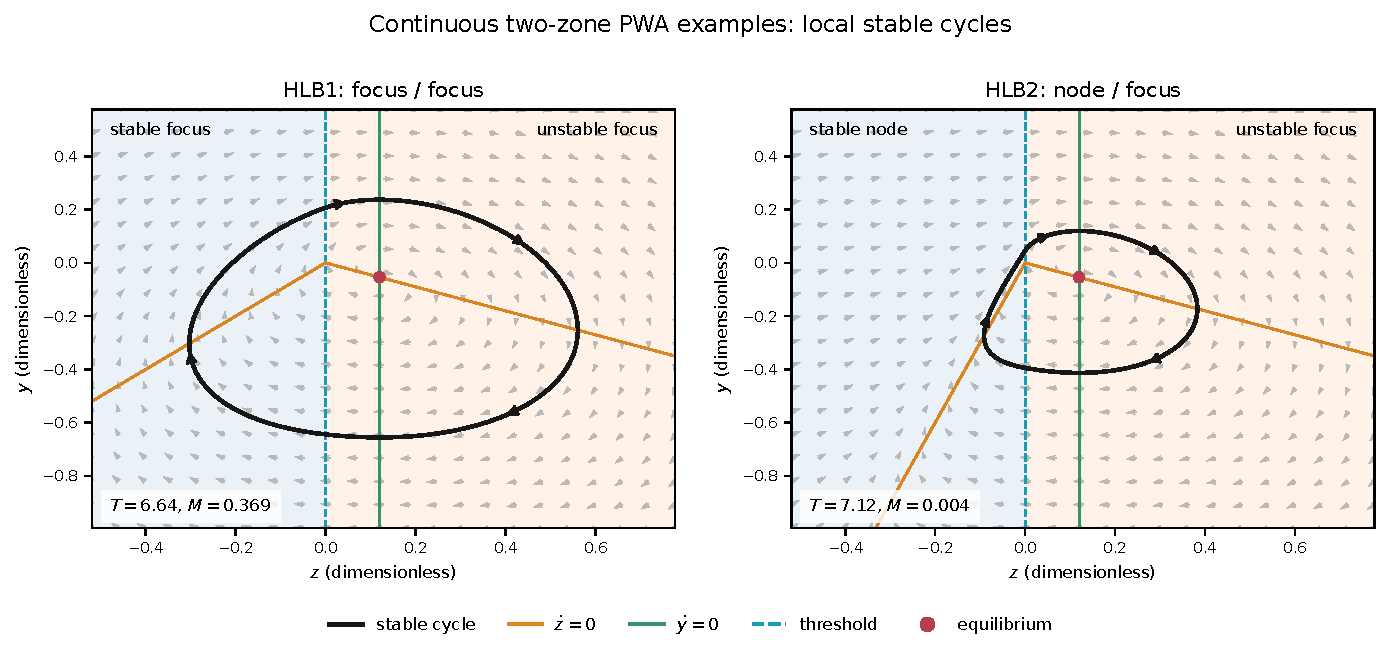
\includegraphics[width=\textwidth,height=.73\textheight,keepaspectratio]{figures/figure3_hlb.pdf}
  \caption{Numerically computed phase portraits for two dimensionless continuous two-zone PWA examples illustrating HLB1 (focus--focus) and HLB2 (node--focus). The system is $\dot z=y-F(z)$, $\dot y=\delta-z$, with $\delta=0.12$, threshold $z=0$, and continuous piecewise-linear $F$ with slopes $(1,-0.45)$ for HLB1 and $(3,-0.45)$ for HLB2. The equilibrium crosses the threshold as $\delta$ passes through zero. The displayed curves are stable periodic orbits; grey arrows show the normalized vector field, and orange and green lines show the nullclines. $T$ is the period and $M$ the nontrivial Floquet multiplier from the divergence integral. The region labels describe the associated affine dynamics; only the red point is the present equilibrium. The examples are constructed and are not fitted Li--Rinzel models.}
  \label{fig:hlb}
\end{figure*}
